\chapter{Experiments}
\label{exp}

In this section I will present methods used to measure word2doc's performance, as well as present certain implementation details
and back up several design decisions with empirical data.

\section{Evaluation Metrics}
\label{exp:eval}

It is hard to accurately measure word2doc's performance because there is no such thing as a designated evaluation dataset working
with Wikipedia articles, or at least I could not find one. There are various document retrieval test sets in existence, such as the
TREC datasets\footnote{\url{https://trec.nist.gov/data.html}}, however these datasets do not work with the Wikipedia corpus, and must
be purchased as well. The SQuAD dataset\footnote{https://rajpurkar.github.io/SQuAD-explorer/} does use the Wikipedia corpus,
however it is a QA dataset and only has 442 unique documents. Most of the data comes from individual queries for different
paragraphs in the documents, not the documents themselves. I judge 442 documents to be too few to contain enough documents to
accurately create context documents, thus training the model on SQuAD will likely not work. Additionally, SQuAD's queries
are QA queries, and because of that they often lack contextual information, or have misleading contextual information. For
example, queries like "How has this foundation changed in recent years?" do not contain any context and are not uncommon throughout
the dataset. For these reasons I chose not to use the SQuAD dataset.

Performing cross-validation is not an option either, because then the net would never have seen certain types of
data. For example, if the net has never been exposed to football related documents, it will not be able to predict the best document
associated with "quarterback". Instead, I have come up with a testing module to create a small sample of hand labeled keyword-document
pairs as described in section \ref{data:eval}. Using this dataset I measure performance on three tasks: the quality of the
\textit{top one} retrieved document, the quality of the \textit{top five} retrieved documents and the quality of the \textit{top
ten} retrieved documents, including their ranking. I measure the quality of the top one document through simple accuracy, and the
quality of the top five and top ten retrieved documents through mean average precision (MAP), as well as through accuracy. As an
evaluation dataset I use W2D-VD-400, and I evaluate word2doc using random samples consisting of 1\% of the Wikipedia corpus. More
to that in section \ref{results}.

A lot of different evaluation metrics exist to measure the performance of IR systems (e.g. precision, recall, F measure,
R-precision, ROC curves, NDCG, MAP). I will explain why I choose MAP instead of other metrics, but first I will quickly
explain the concepts of precision and recall because they are relevant.

\paragraph{Precision}
Precision ($P$) is the fraction of retrieved documents that are relevant:

\begin{gather}
  Precision = \frac{\#(\text{relevant items retrieved})}{\#(\text{retrieved items})} = P(\text{relevant}|\text{retrieved}) =
  \frac{tp}{tp + fp}
\end{gather}

where $tp$ is true positive and $fp$ is false positive.

\paragraph{Recall}
Recall ($R$) is the fraction of relevant documents that are retrieved:

\begin{gather}
  Recall = \frac{\#(\text{relevant items retrieved})}{\#(\text{relevant items})} = P(\text{retrieved}|\text{relevant}) =
  \frac{tp}{tp + fn}
\end{gather}

where $tp$ is true positive again and $fp$ is false positive again, and $fn$ is false negative.

\paragraph{F Measure}

F measure is a single measure that trades off precision versus recall. In fact, it is the weighted harmonic mean of precision and
recall, and one of the most widely used performance metrics for IR tasks:

\begin{gather}
  F = \frac{1}{\alpha \frac{1}{P} + (1 - \alpha) \frac{1}{R}} = \frac{({\beta}^2 + 1)PR}{{\beta}^2P + R} \quad \text{where} \quad
  {\beta}^2=\frac{1 - \alpha}{\alpha}
\end{gather}

where $\alpha \in [0, 1]$ and $\beta \in [0,\infty]$. The most common F measure is the $F_1$ measure, which equally weights precision
and recall, making $\alpha = 1/2$ or $\beta = 1$. The $1$ in $F_1$ refers to the $\beta$ value, and is short for $F_{\beta = 1}$.
When using $\beta = 1$, the above formula simplifies to:

\begin{gather}
  F_1= \frac{2PR}{P + R}
\end{gather}

However, we don't have to use an equal weighting. When $\beta < 1$, precision is emphasized, and when $\beta > 1$, recall is
emphasized. Thus, a value of $\beta = 3$ or $\beta = 5$ might be used if recall is more important, and a value of $\beta = 1/2$
when precision is more important.

F measure is popular because it trades off two opposing metrics. For instance, you can get a recall of one by returning all
documents, however that yields a low precision, and vice-versa. Finding a trade off between these two metrics is a good way of
measuring the overall performance of an IR system. However, it does require to calculate the recall, and that is often a problem in
large data sets. Recall is the fraction of relevant documents that are retrieved, so in order to calculate recall you need to know the
set of all relevant documents for a given query. That is very hard to calculate in large sets such as Wikipedia. Instead,
it is possible to estimate recall by taking samples of the dataset, or by adhering to golden standards for a dataset, if such are
available \citep{manning2009}. However, since I am evaluating word2doc on a subset of the full dataset I have no golden standard
available, and taking a sample of the sample to estimate recall does not seem to yield accurate results. Thus, I discarded all
metrics using recall or that requires similar knowledge as recall, such as ROC curves or R-precision.

Furthermore, F measure does not take the order of a ranking into account, and applying it to a single returned document is
useless (precision and recall assume there is a set of relevant documents greater than one). Thus, it does not make sense to
apply F measure to either of my two evaluation tasks. Instead, I turned to MAP, which is a standard metric to measure the
quality of a ranking.


\subsection{Mean Average Precision}
\label{exp:map}

According to \citet{manning2009}, MAP is the most common metric to measure performance in the \textit{TREC} community. Like the
F measure, MAP also provides a single-figure measure of quality for all queries. It does this across all levels of recall and has
been shown to have especially good discrimination and stability \citep{manning2009}. For a single query, average precision is the
average of the precision value obtained for the top $k$ documents remaining, after each document is removed from the set one after
the other. This value is then averaged over all queries. More specifically, if the set of relevant documents for a query $q_j \in
Q$ is ${d_1,...,d_{mj}}$ and $R_{jk}$ is the set of ranked retrieval results from the top to document $d_k$, then

\begin{gather}
  MAP(Q) = \frac{1}{|Q|}\displaystyle\sum_{j=1}^{|Q|} {\frac{1}{m_j} \displaystyle\sum_{k=1}^{m_j}{\text{Precision}(R_{jk})}}
\end{gather}

MAP is a rough estimate of the area under the precision-recall curve for a set of queries $Q$. The precision-recall curve is a graph
in which precision is mapped against recall. It has often a saw-tooth shape which occurs the following way: If the $n^{th}$
document retrieved is useful, both precision and recall increase, but if it is not, recall stays the same but precision drops,
resulting in a saw-tooth like shape.

Furthermore, MAP weights higher ranked documents much more heavily than lower ranked documents, because of the way precision
works. With only one document precision is either 0 or 1. If we add a second document which is not relevant, and assuming the first
document was relevant (precision = 1), than precision drops to 0.5, and so on. Thus, the first document alone having a precision
of one is weighted twice as much as the first and second documents combined, which have a precision of 0.5. MAP thus has a natural
way to give more attention to more relevant documents.

MAP scores can strongly vary, but the higher the score, the better the system performs. A good score is usually somewhere between 0.5
and 0.7. However, it should be noted that MAP scores can vary widely across different queries, sometimes between 0.1 and 0.7 and
that test data needs to be large and diverse enough to yield a representative score.

To calculate MAP scores, I built an evaluation system (\textit{evaluation.py}) which presented me pairwise with the query and the
document in question. I then judged whether the document in question was relevant to the query. I did this for all ranked documents
for all queries, and the system evaluated MAP scores out of my judgments. It should be noted that my judgments are not bias free,
and in order to gain more accurate results with less bias, a system like Amazon Mechanical Turk could be used.

\section{Implementation Details}

In this section I cover relevant implementation details. I present the hyperparameters used while training the final model
presented in this thesis, as well as mention a few steps I took to improve final results. I also explain how I trained
subsets of the full Wikipedia data, and talk about some problems that come with that.

\subsection{Hyperparameters}
\label{exp:hyppar}

As I will explain in section \ref{results}, I only trained word2doc on 1\% of the full Wikipedia dataset. The hyperparameters used
train the word2doc neural net on that 1\% ($58,170$ documents) can be found in Table \ref{tbl:w2d-hyp}.

\begin{table}[H]
  \centering
  \begin{tabular}{|p{6cm}|p{4cm}|}
    \hline
    \multicolumn{2}{|c|}{W2D Network Hyperparameters} \\
    \hline
    Parameter&Value \\
    \hline
    \hline
    epochs & 30 \\
    batch size &2096 \\
    input dimension & 4096 \\
    embedding dimension & 512 \\
    embedding vocab size & 581700 \\
    num\@. context docs & 10 \\
    dropout rate & 0.3 \\
    loss function & negative sampling \\
    negative sampling sample size & 10 \\
    optimizer & adam \\
    adam learning rate & 0.001 \\
    adam beta1 & 0.9 \\
    adam beta2 & 0.999 \\
    adam epsilon & 1e-08 \\
    \hline
  \end{tabular}
  \caption{W2D Hyperparameters}
  \label{tbl:w2d-hyp}
\end{table}

The \textit{input dimension} refers to the InferSent embedding, which has a dimension of 4096. The \textit{embedding dimension} is
the dimension of the document embedding vectors. The embeddings are relatively low dimensional as explained earlier in section
\ref{theory:embb}. The \textit{embedding vocab size} is the number of documents for which an embedding was learned. This is not
equal to 58170 because for each of the 5000 documents, 10 documents were chosen as context, so $58170 * 10 = 581,700$. There is
some overlap between documents, but since we don't know how much, I kept it at $581,700$. However, there is no impact if there are
too many document
embeddings, some will just not be used. The \textit{num\@. context docs} refers to the number of context documents word2doc uses,
which is ten. \textit{negative sampling sample size} is the number of documents used to update the weights in a "negative" direction
during negative sampling, as explained in section \ref{theory:negsamp}. Furthermore, Dropout \citep{dropout} was used with a rate of
0.3 to further improve results. And last but not least, the adam values refer to the hyperparameters used for the adam optimizer
\citep{adam}.


\subsection{Shuffling Context Documents}

Shuffling the order in which the network sees context documents in each run turned out to be very important. Without shuffling
context documents before each iteration, the model dropped from a 0.99\% accuracy on a 5000 document sample to a 22.46\% accuracy
on the same sample when it was presented context documents in a different order than that which it learned. This strongly
suggests the model was memorizing the order in which it was presented context documents. Once context documents were shuffled
before each iteration, the net stopped memorizing, and scored a 0.99\% accuracy on the training set, regardless of the order
the context documents were in.

\subsection{Training on Subsets}

When training on subsets of the full Wikipedia corpus a central problem arises: Not all context documents from the full Wikipedia
corpus are contained in the random subsample. In fact very few data points contain all context documents. It is also not possible
to add the context documents to the subsample without using the full Wikipedia corpus for the following reason: If I train on a
sample of 5000 documents, then there are around $5000 * 10 = 50,000$ context documents, as explained above. If these 50,000
documents were then added to the sample, I would need ten documents again for each new document added, resulting in $~500,000$ new
documents to add, again. This will continue until the entire Wikipedia set has been added to the sample.

To mitigate this problem, I replaced missing context documents with duplicates of existing ones. This means that for all tests
presented in this thesis, I was unable to exploit the full potential of context documents as I never trained on the full Wikipedia
corpus. It is possible that results improve significantly when trained using all context documents.


\section{Performance of Design Decisions}

Now I will delve into the impact certain design decisions have on the model as a whole, give an intuition for what is happening
wherever relevant, and back up my intuition with empirical data that I gathered while testing the model.

\subsection{Document Embeddings}
\label{exp:embb}

As I briefly mentioned in section \ref{theory:w2d-net}, when training word2doc, document embeddings are automatically trained
alongside. The context documents word2doc uses are turned into embeddings, and this can be visualized. It serves as a good illustration
for what word2doc is learning. Figure \ref{fig:tsne} is a 3-D representation of 2000 document embeddings created using t-SNE
\citep{tsne}, a visualization algorithm for high dimensional data. They originate from sample training data consisting of 200
documents. Each document has ten context documents, and since there is almost no overlap between context documents as it is extremely
unlikely all context documents occur in a random 200 sized sample of Wikipedia, we can multiply 200 by ten, and get 2000.

\begin{figure}
  \begin{center}
    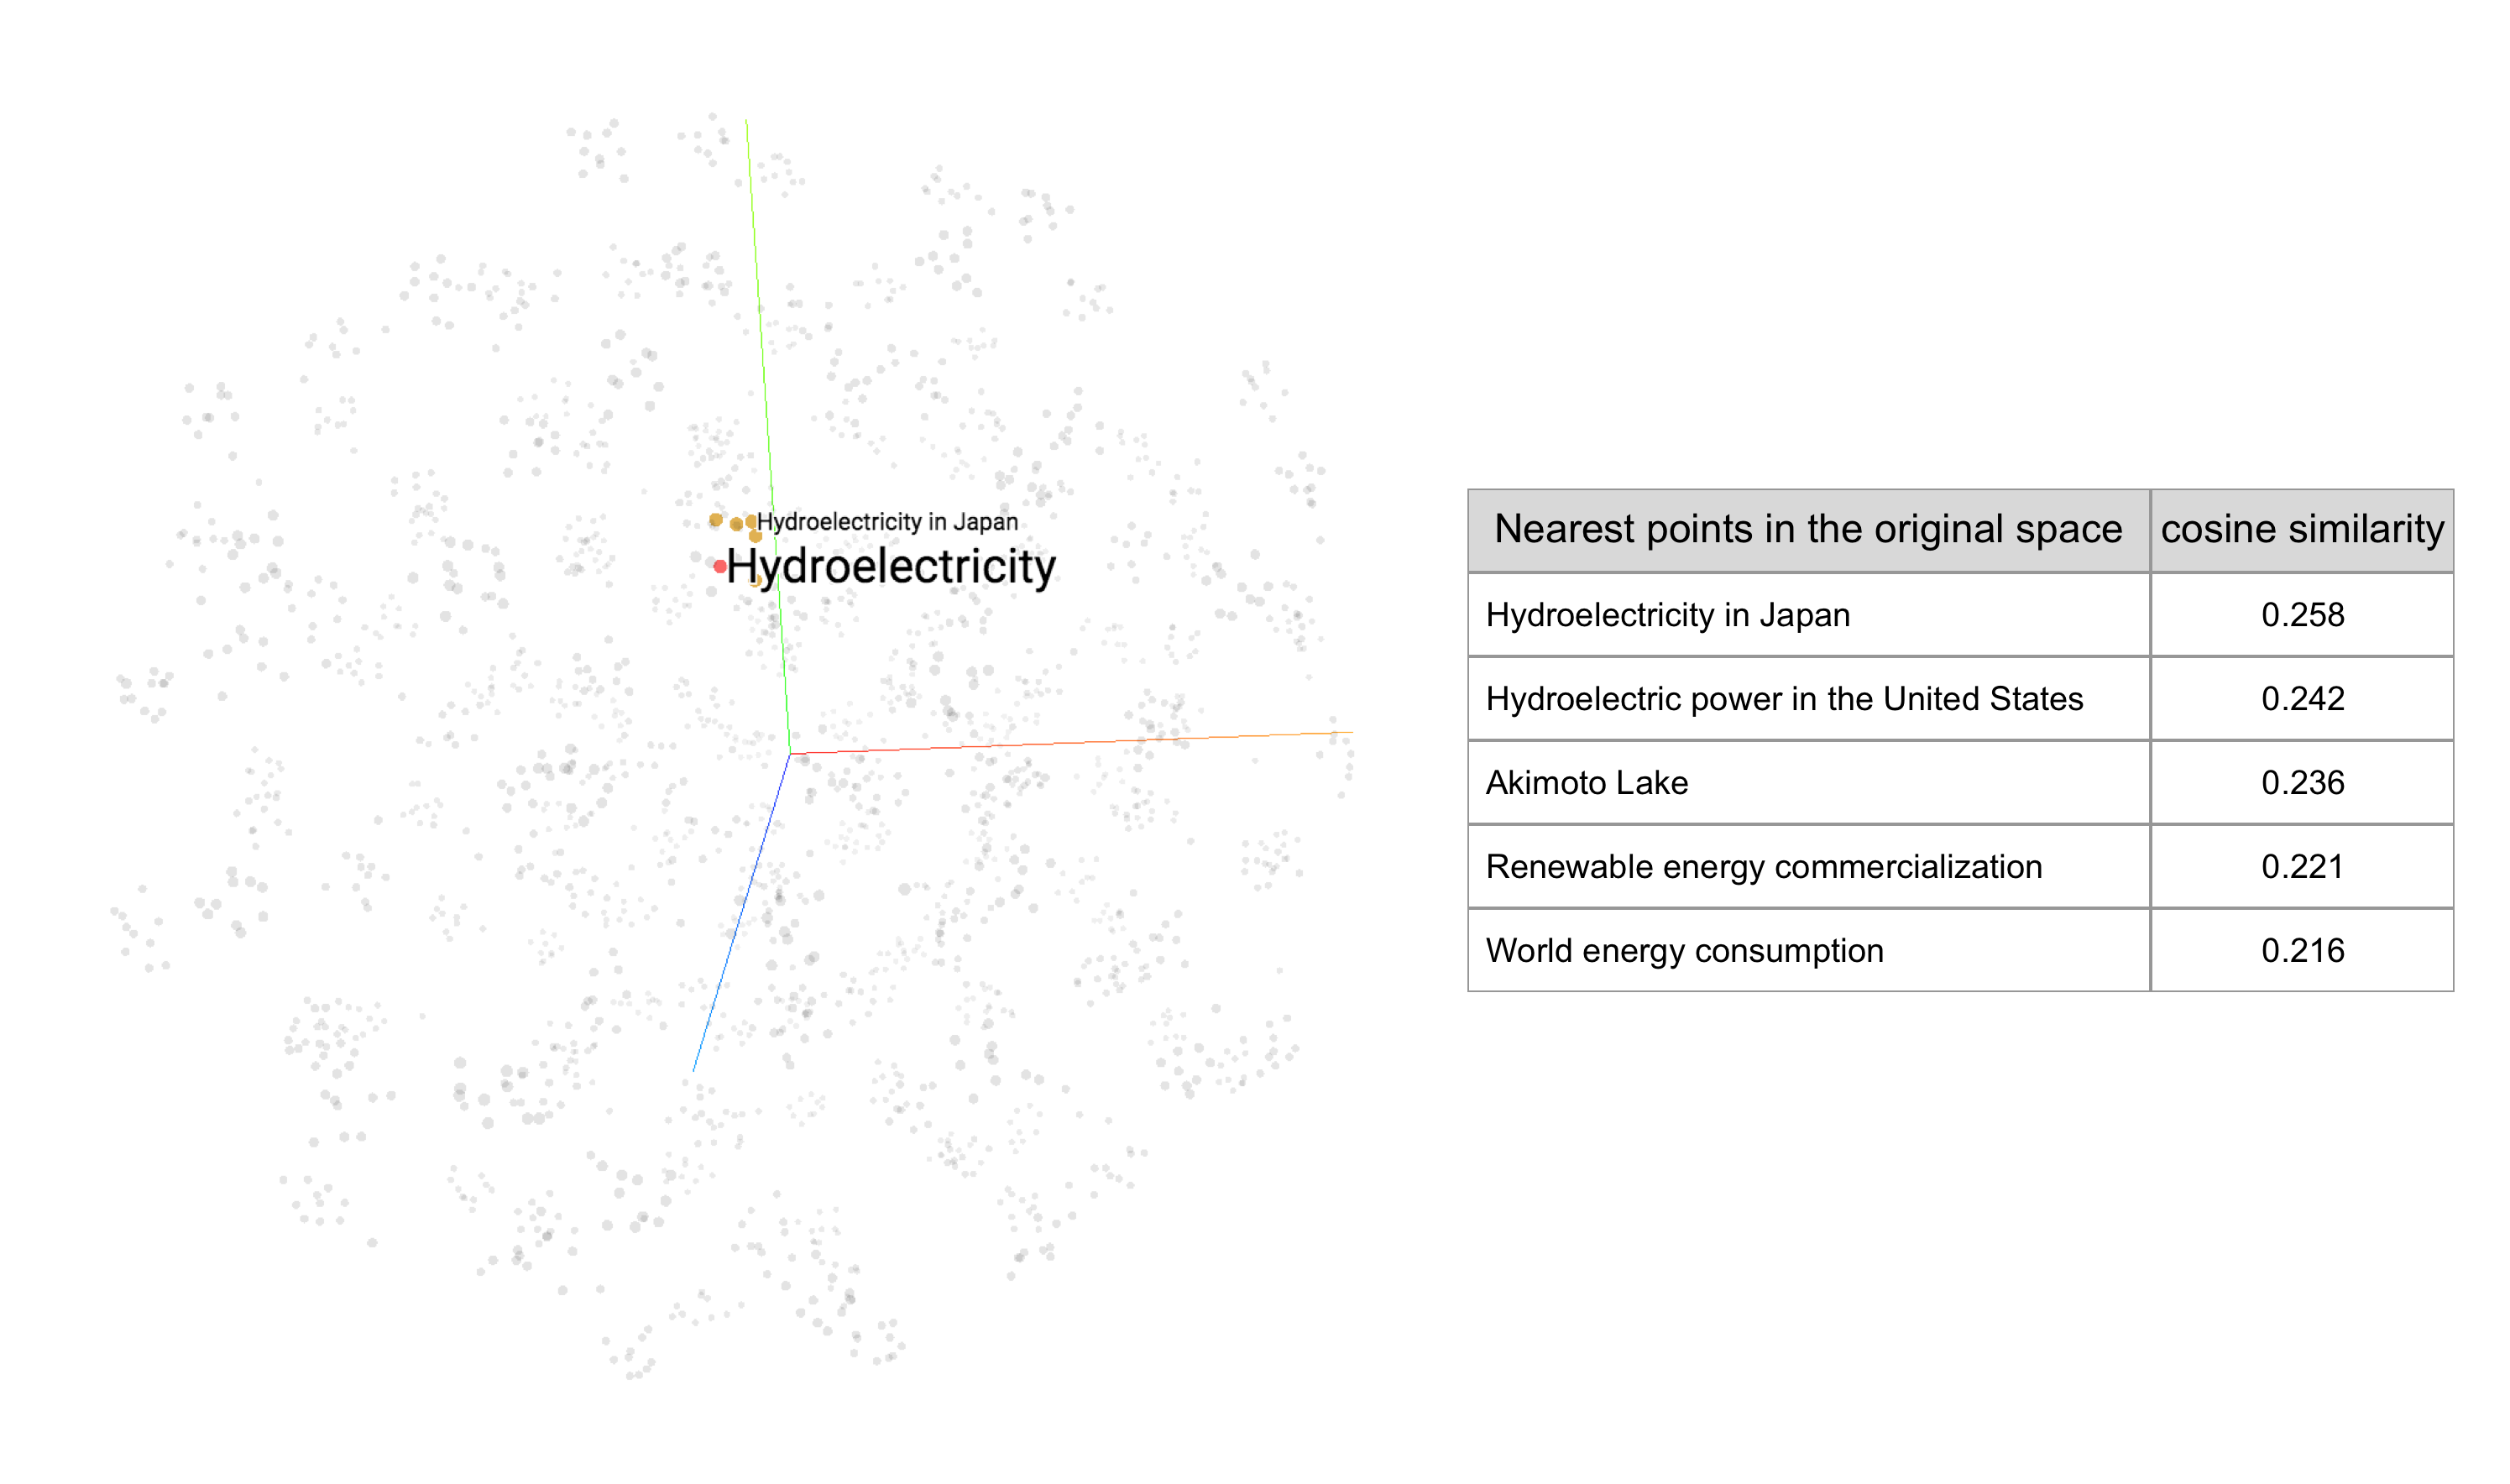
\includegraphics[scale=0.13]{emb.png}
  \end{center}
  \captionsetup{width=.75\linewidth}
  \caption{A visualization of 2000 document embeddings using t-SNE \citep{tsne} trained on 200 data points, along with the five
  closest points to "Hydroelectricity".}
  \label{fig:tsne}
\end{figure}

As can be seen from the visualization, clear clusters form. Each point represents a document, and each cluster of documents
shares similar context. Highlighted are the five documents closest to "Hydroelectricity" in the original space, measured by cosine
similarity as explained in section \ref{theory:cosinesim}. It is apparent that the top five documents all have something to do with
hydroelectricity (Akimoto Lake is used for the generation of hydroelectricity).

It should be noted, that these documents are only chosen among 2000 documents, not the full Wikipedia corpus. This means the
results are limited by the number of documents available. Unfortunately, when already as many as 50,000 documents are visualized,
clear clusters disappear, and instead only a huge sphere remains. However, when scaling from 2000 to 50,000 documents,
the performance is not impaired, both models reaching a training accuracy of 99.9\%, and the later reaching a testing accuracy
of 69.3\%. Since visualizing embeddings for 50,000 documents is already a problem, visualizing the full Wikipedia dataset will probably
not work very well either.

This visualization shows that word2doc is definitely learning something. The document embeddings are formed correctly and
encapsulate semantic meaning of each document. Occasionally clusters form that are only very loosely connected through context, and
sometimes have nothing to do with each other, but in general clusters that form share similar contexts.


\subsubsection{t-SNE Visualization}

There are a few points to make about t-SNE \citep{tsne}, the algorithm used to visualize the document embeddings, because it can
be misleading. t-SNE performs a dimensionality reduction for modeling high-dimensional data faithfully in two or three dimensions,
similar to PCA. However, unlike PCA, it is non-linear and adapts to the underlying data, performing different transformations on
different regions. It has two hyper parameters, the learning rate (or "epsilon") and perplexity.

As the sklearn documentation puts it \footnote{\url{http://scikit-learn.org/stable/modules/generated/sklearn.manifold.TSNE.html}}:
"The learning rate for t-SNE is usually in the range [10.0, 1000.0]. If the learning rate is too
high, the data may look like a ‘ball’ with any point approximately equidistant from its nearest neighbors. If the learning
rate is too low, most points may look compressed in a dense cloud with few outliers." To create the graph above, I used a learning
rate of 10 and a perplexity of 15.

The perplexity is a bit more tricky. It is a guide on how to balance attention between local and global aspects of the data.
In a way it guesses how many close neighbors each point has. The authors of the paper say, “The performance of t-SNE is fairly robust to
changes in the perplexity, and typical values are between 5 and 50.” \citep{tsne} However, the reality is more complex. Changes in perplexity
can have huge effects on the visualization. Random data can, with the right hyperparameters, be shown to have certain clusters,
which is impossible since it is random. Visualizations can differ from across different runs and cluster size is not always
meaningful. Overall results offered by t-SNE are not straight forward to interpret.

To make sure the visualization from Figure \ref{fig:tsne} is somewhat accurate, I ran different versions, each for 5000 iterations as
it was suggested in the guide presented by TensorFlow\footnote{\url{https://distill.pub/2016/misread-tsne/}}.
Fixing the perplexity at the default (12) and testing learning rates of 2, 10, 50 and 100, I noticed that at a learning rate of
ten the model reached a point of stability. To determine perplexity, I fixed the learning rate at ten and tested multiple perplexities,
starting at five and incrementing perplexity by five at every step. From 15 and on, I did not see a big change in the visualization, and
thus I stuck with a learning rate of 10 and a perplexity of 15.


\subsection{A Deeper Look}
\label{exp:dl}

In order to get a better grasp of the impact certain design decisions have on the final model, I built different versions of the
model, each version testing one design decision. More specifically, I tested the impact of averaging context documents and query
versus concatenating them. I also tested the impact of the data augmentation scheme from section \ref{data:overfitting} and finally I
tested the impact that the use of context documents has on the final results.

Word2doc as it has been presented thus far, that is with averaging, serves as a baseline for the tests to come. Each model was
trained on a subset of 5000\footnote{Testing on a significantly larger data set would have yielded more accurate results, however it
would not have been feasible.} randomly chosen documents out of the entire Wikipedia corpus, and evaluated on W2D-VD-200.
All hyper parameters are the same as the ones presented in Table \ref{tbl:w2d-hyp}, except for the number of epochs and batch
size which change on each run according to the table in Figure \ref{fig:w2d-model-tests}

\begin{figure}
  \begin{center}
    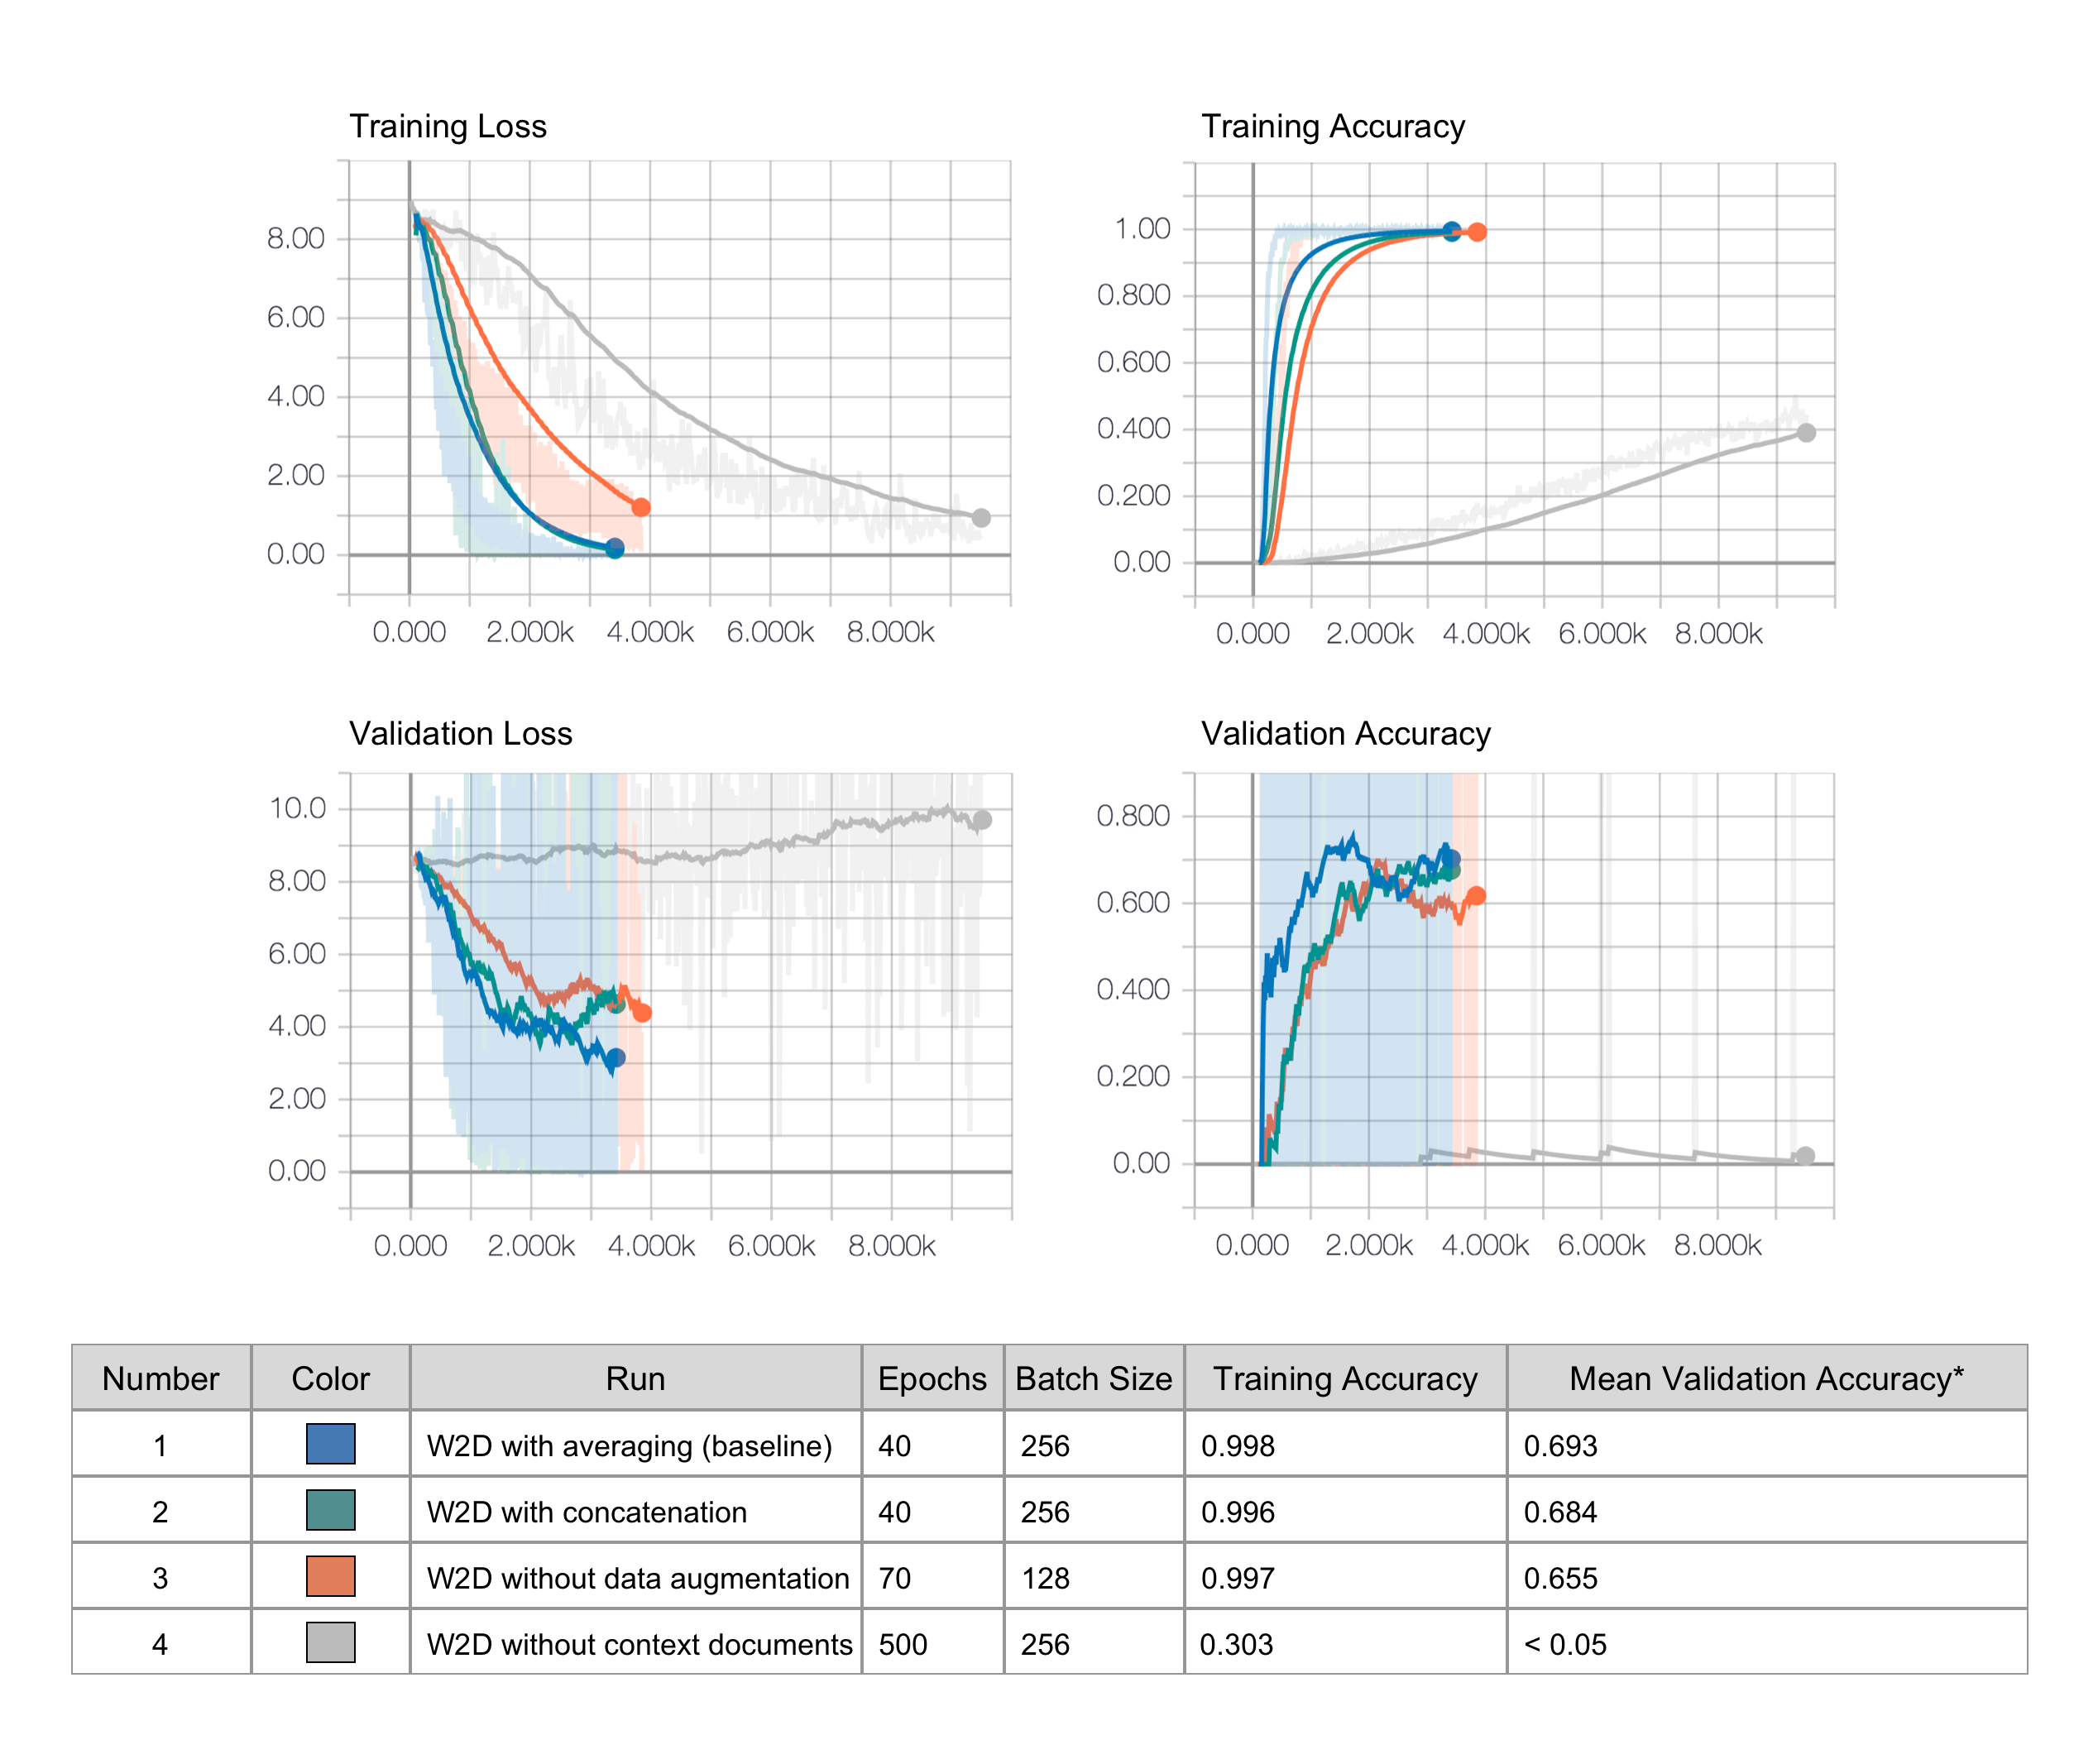
\includegraphics[scale=0.18]{alternative-w2d-versions.png}
  \end{center}
  \caption{Results on four different models}
  \label{fig:w2d-model-tests}
\end{figure}

\paragraph{Baseline}
All runs are compared with the baseline. For each run, every feature is fixed, except for the one that is being
tested. For example, run no. 2 makes use of concatenation instead of averaging, but still uses data augmentation. Run no. 3 does
not make use of data augmentation, but does use averaging, etc.

\paragraph{W2D with concatenation}
In this run I compare concatenation with averaging, in terms of which function to apply to all document embeddings along with the
reduced query tensor (Figure \ref{fig:w2d}).

Word2doc using concatenation performs slightly worse compared to the baseline model. However, given that these tests are only
performed on 5000 documents, it is not necessarily clear whether this slight underperformance is reproducible on the entire dataset.
However, it is clear that the baseline model learns faster than the concatenation model. The baseline's training accuracy as well
as its validation accuracy both have steeper slopes than the training and validation accuracies of the concatenation model, and
that is mainly why I chose to average over concatenation.

A possible explanation for this speedup could be that averaging results in a much smaller tensor (size 512) compared to
concatenation. Therefore there are a lot less weights to be learned, and thus the model trains faster. The question arises of whether the
smaller number of weights is still sufficient for a much larger dataset, where the model does not have to choose between 5000 but
between 5 million documents. Intuitively I would say yes, because $512^3$ is already $134,217,728$, but since weights are real
numbers and thus have many more than 3 possible configurations, 512 weights should be more than enough to semantically encode 5
million documents.

\paragraph{W2D without data augmentation}
In this run, I compare the baseline model that uses data augmentation with the baseline model that does not use data augmentation.
Not making use of data augmentation means that only the Wikipedia title is taken as a query. Therefore, without data augmentation there are
exactly 5000 data points to train on, compared to the usual 24,488 data points that are obtained through data augmentation. In
order to compensate, I increased the number of epochs and reduced the batch size. Given these changes, word2doc without data
augmentation performed slightly worse. It is difficult to say to what degree this effect is reproducible on the full data set,
and how much influence the change in hyper-parameters had but the effect does seem to be only small.

It is also possible that the full benefit of data augmentation only becomes apparent with very large corpora, as that is where
documents and queries can intertwine the most, leading to better document embeddings. Perhaps with 5000 documents the data
augmentation scheme does not create enough useful connections between queries and documents to better reflect the semantic
meaning of a query or document, which then would only have little effect on the document embeddings.

\paragraph{W2D without context documents}
Now I test the impact that document embeddings as a whole have on the model. To do so, I removed the document retriever and
everything to with it from word2doc, similar to PV-DM and PV-DBOW in paragraph vectors \citep{doc2vec}. What is left behind
can be seen in Figure \ref{fig:w2d-raw}

\begin{figure}
  \begin{center}
    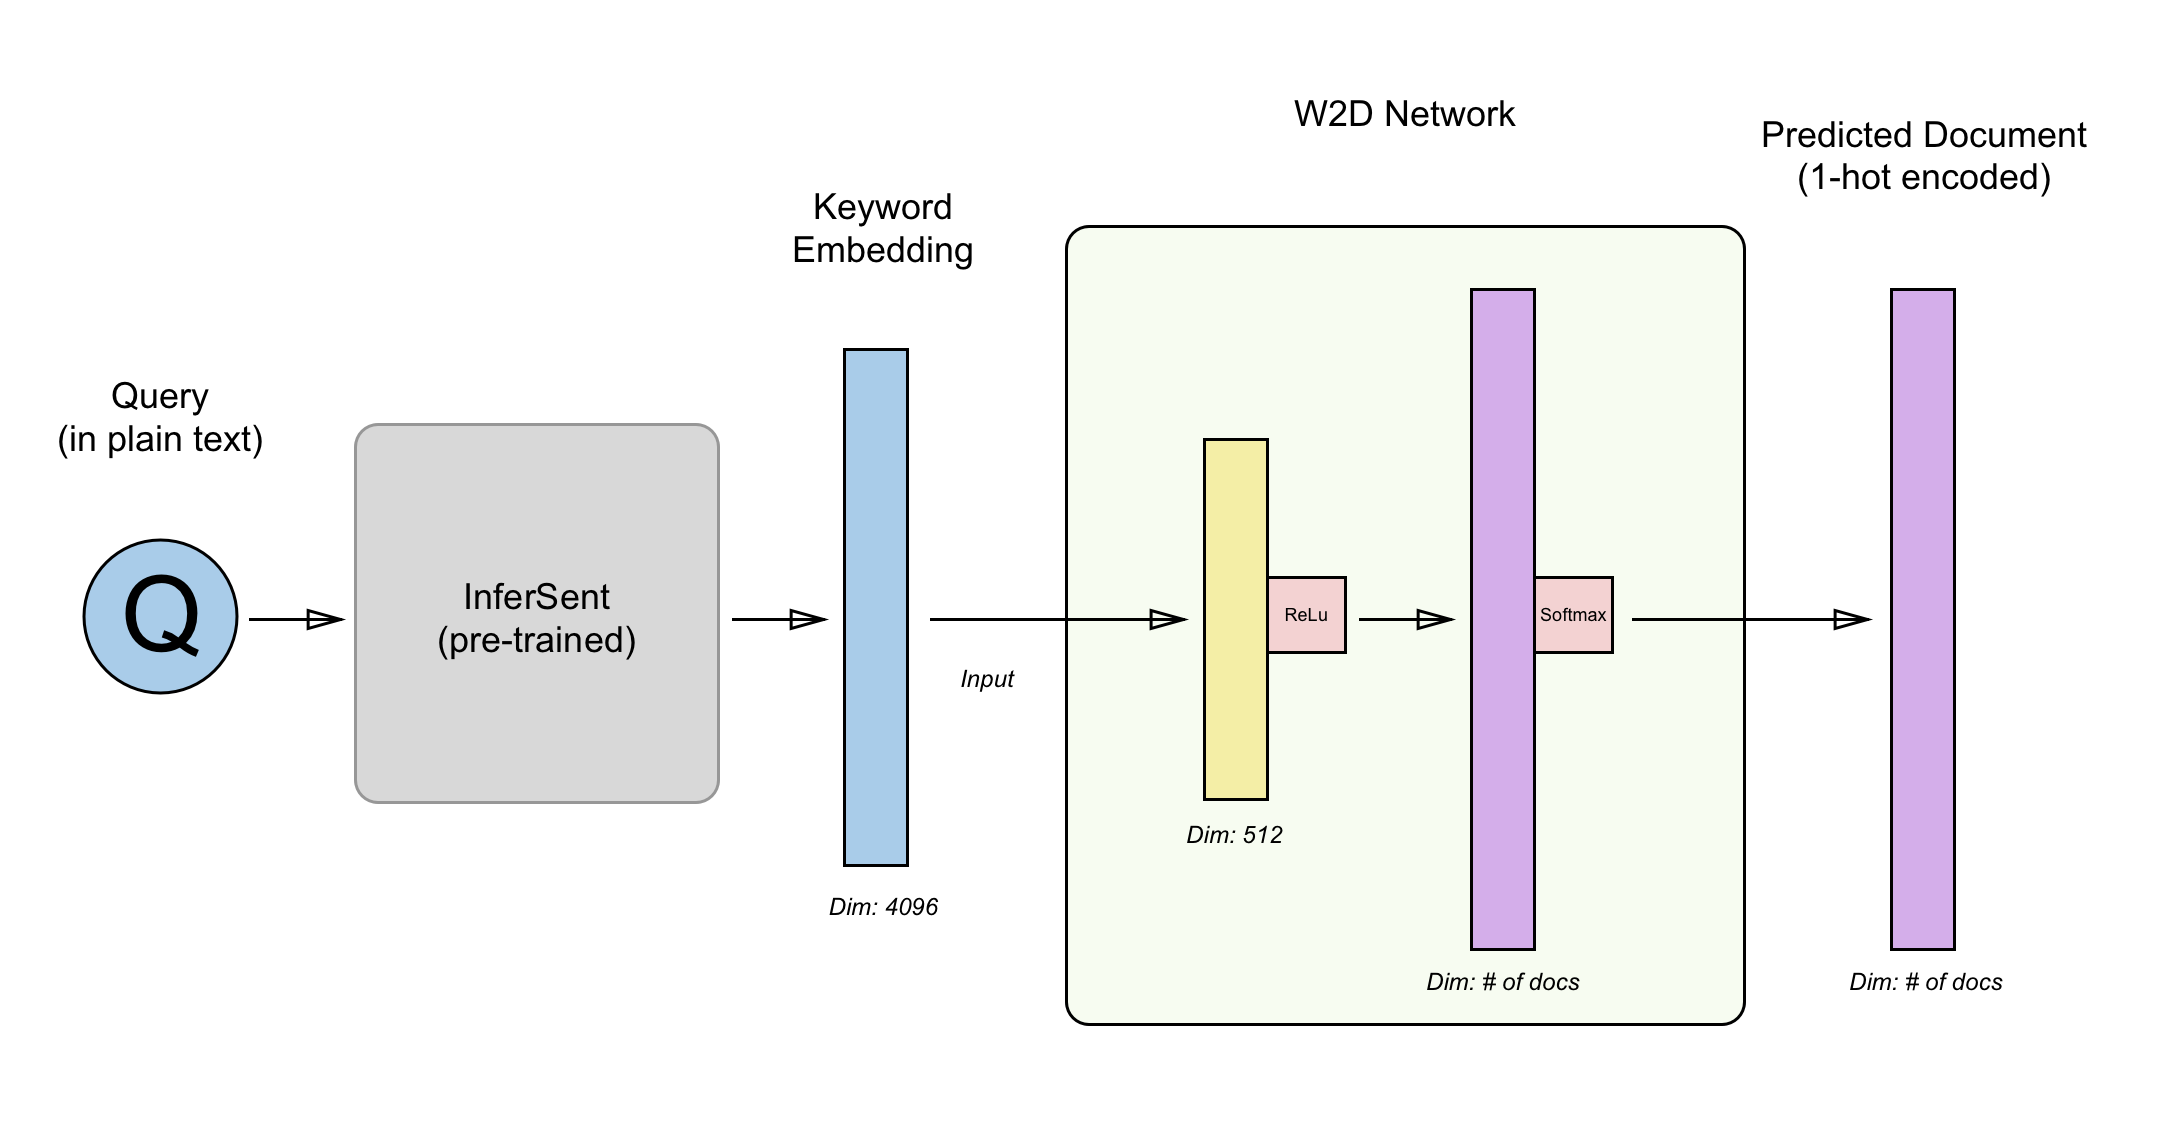
\includegraphics[scale=0.17]{W2D.png}
  \end{center}
  \caption{W2D Architecture without context documents}
  \label{fig:w2d-raw}
\end{figure}

However, given this change, the model learns much slower. In fact after 500 epochs, the adapted model only reached a training
accuracy of about 30\%, and a validation accuracy of less than 5\%. In fact the model did not seem to learn at all. This
implies that the network is very reliant on the context documents. Either it memorizes the context documents despite dropout and
fixed document embeddings, or it is able to generalize using the context documents. However, the fact that the other models achieve
validation accuracies of around 68\%, and the fact that the embeddings are clearly learned as can be seen from Figure \ref{fig:tsne}
suggest that the model does in fact generalize, at least to a certain degree.

